\subsection{Image Degradation and Restoration}

Figur~\ref{fig:degradation-restoration-process} viser selve processen, som vi vil gå igennem.\\
Nedbrydningsfunktionen $(H)$, som med støj $(\eta)$ laver et nedbrydt billede $(g)$. \\
Givet $g$ og viden om nedbrydningsfunktionen $H$ og den støj $\eta$ er målet at restaureringen at finde et estimeret $\hat{f}$ af de originale billede.

\begin{figure}[h]
	\centering
	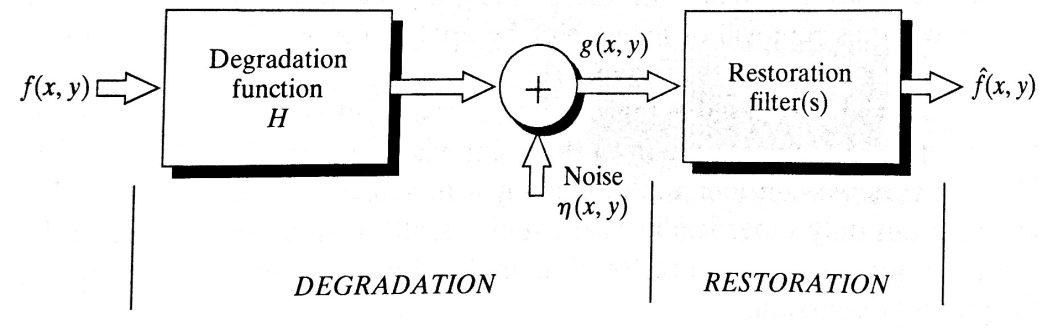
\includegraphics[width=0.9\linewidth]{figs/spm06/degradation-restoration-process}
	\caption{Illustration af degradation/restoration processen.}
	\label{fig:degradation-restoration-process}
\end{figure}

Da $H$ er lineær vil det nedbrudte billede i det spatiale domæne være givet ved ligningen vist i Figur~\ref{fig:degradation-spatial-eq}. 

\begin{figure}[h]
	\centering
	
\includegraphics[width=0.7\linewidth]{figs/spm06/degradation-spatial-eq}
	\caption{Ligning for det nedbrudte billede i det spatiale domæne, hvor stjernen er ''convolution'' og h(x,y) er degradation funktionen.}
	\label{fig:degradation-spatial-eq}
\end{figure}

Da vi ved at convolution i det spatiale domæne svare det multiplikation i frekvensdomænet kan vi opstille ligningen vist i Figur~\ref{fig:degradation-freq-eq}.

\begin{figure}[h]
	\centering
	
\includegraphics[width=0.7\linewidth]{figs/spm06/degradation-freq-eq}
	\caption{Ligning for det nedbrudte billede i frekvensdomænet, hvor de store bogstaver repræsentere Fouriertransformationen af termerne i Figur~\ref{fig:degradation-spatial-eq}.}
	\label{fig:degradation-freq-eq}
\end{figure}
